\documentclass[12pt,a4paper]{article}
\usepackage[utf8]{inputenc}
\usepackage[T1]{fontenc}
\usepackage{amsmath}
\usepackage{amsfonts}
\usepackage{amssymb}
\usepackage{graphicx}
\usepackage[width=0.00cm, left=3.00cm, right=2.00cm, top=3.00cm, bottom=2.00cm]{geometry}
\usepackage{tikz}
\title{Lista Extra 3}
\date{}
\begin{document}
	\maketitle
	\begin{center}
		\textbf{Exercícios para aula}\\
		\textbf{Exercícios de Esperança e Função de V.A. 19/09/2022}
	\end{center}
	1) Uma fábrica produz válvulas, das quais 20\% são defeituosas. As válvulas são vendidas em caixas com 10 peças. Se a caixa não tiver nenhuma defeituosa, eu preço de venda é R\$10,00, tendo uma o preço é R\$8,00, duas ou três o preço é R\$ 5,00 e, mais de três o preço é R\$2,00. Qual o preço médio de uma caixa?
	\vspace{1cm}\\
	X$\sim$Bin\{10; 0,2\}
	\vspace{1cm}
	\begin{center}
		$\mathbb{P}$(X = 0) = $\dbinom{10}{0} * 0,2^0 * 0,8^10 = 0,1074$
		\vspace{1cm}\\
		$\mathbb{P}$(X = 1) = $\dbinom{10}{1} * 0,2^1 * 0,8^9 = 0,0268$
		\vspace{1cm}\\
		$\mathbb{P}$(X = 2) = $\dbinom{10}{2} * 0,2^2 * 0,8^8 = 0,0067$
		\vspace{1cm}\\
		$\mathbb{P}$(X = 3) = $\dbinom{10}{3} * 0,2^3 * 0,8^7 = 0,0017$
		\vspace{1cm}\\
		$\mathbb{P}$(X > 3) = 1 - $\mathbb{P}$(X $\leq$ 3) = 1 - (0,1074 + 0,0268 + 0,0067 + 0,0017)
		\vspace{0.25cm}\\
		$\mathbb{P}$(X > 3) = 1 - 0,3838 = 0,6162
	\end{center}
	\vspace{1cm}
	Y = Preço da caixa
	\vspace{1cm}\\
	\begin{center}	
		E(Y) = 10 * 0,1074 + 8 * 0,0268 + 5 * (0,0067 + 0,0017) + 2 * 0,6162
		\vspace{0.25cm}\\`
		E(Y) =  1,074 + 0,2144 + 4,2 + 1,2324 = 6,7208
		\vspace{1cm}\\
		O preço médio da caixa é R\$6,72
	\end{center}
	\vspace{1cm}
	2) Um jogo consiste em retirar duas bolas, uma a uma, sem reposição de uma caixa que contém 4 bolas brancas, 4 pretas e 2 vermelhas. Suponha que o indivíduo ganhe R\$20,00 para cada bola preta selecionada, R\$10,00 para cada bola branca e R\$30,00 para cada bola vermelha escolhida. Seja X = número de bolas vermelhas escolhidas.\\
	a) Encontre a distribuição de probabilidade de X.\\
	\vspace{1cm}\\
	\begin{center}
		\begin{tikzpicture}
			\tikzstyle{level 1} = [sibling distance=6cm, level distance=2cm]
			\tikzstyle{level 2} = [sibling distance=2cm, level distance=3cm]
			\node{}
				child{
				node{B}
				child{
					node{B}
					edge from parent
					node[fill=white]{\(\dfrac{3}{9}\)}
				}
				child{
					node{P}
					edge from parent
					node[fill=white]{\(\dfrac{4}{9}\)}
				}
				child{
					node{V}
					edge from parent
					node[fill=white]{\(\dfrac{2}{9}\)}
				}
				edge from parent
				node[fill=white]{\(\dfrac{4}{10}\)}
				}
				child{
				node{P}
				child{
					node{B}
					edge from parent
					node[fill=white]{\(\dfrac{4}{9}\)}
				}
				child{
					node{P}
					edge from parent
					node[fill=white]{\(\dfrac{3}{9}\)}
				}
				child{
					node{V}
					edge from parent
					node[fill=white]{\(\dfrac{2}{9}\)}
				}
				edge from parent
				node[fill=white]{\(\dfrac{4}{10}\)}
				}
				child{
				node{V}
				child{
					node{B}
					edge from parent
					node[fill=white]{\(\dfrac{4}{9}\)}
				}
				child{
					node{P}
					edge from parent
					node[fill=white]{\(\dfrac{4}{9}\)}
				}
				child{
					node{V}
					edge from parent
					node[fill=white]{\(\dfrac{1}{9}\)}
				}
				edge from parent
				node[fill=white]{\(\dfrac{2}{10}\)}
				};
		\end{tikzpicture}
	\end{center}
	\vspace{1cm}
	\[
	S_{X} =
	\begin{cases}
		(B, B); (B, P); (P, P); (P, B) = 0\\
		(B, V); (P, V); (V, B); (V, P) = 1\\
		(V, V) = 2
	\end{cases}
	\]
	\vspace{1cm}\\
	\begin{center}
		$\mathbb{P}$(X = 0) = $2 * \left(\dfrac{4}{10} * \dfrac{3}{9}
		+ \dfrac{4}{10} * \dfrac{4}{9}\right) = \dfrac{56}{90}$
		\vspace{1cm}\\
		$\mathbb{P}$(X = 1) = $2 * \left(\dfrac{4}{10} * \dfrac{2}{9}
		+ \dfrac{2}{10} * \dfrac{4}{9}\right) = \dfrac{32}{90}$
		\vspace{1cm}\\
		$\mathbb{P}$(X = 2) = $\dfrac{2}{10} * \dfrac{1}{9} = \dfrac{2}{90}$
	\end{center}
	\vspace{1cm}
	b) Quanto, em reais, se espera ganhar nesse jogo?\\
	\vspace{1cm}\\
	Y = Dinheiro ganho no jogo\\
	\vspace{1cm}\\
	\[
	S_{Y} =
	\begin{cases}
	(B, B) = 20\\
	(B, P); (P, B) = 30\\
	(P, P); (B, V); (V, B) = 40\\
	(P, V); (V,P) = 50\\
	(V, V) =60\\
	\end{cases}
	\]
	\vspace{1cm}\\
	\begin{center}
		$\mathbb{P}$(Y = 20) = $\dfrac{4}{10} * \dfrac{3}{9} = \dfrac{12}{90}$
		\vspace{1cm}\\
		$\mathbb{P}$(Y = 30) = $2 * \left(\dfrac{4}{10} * \dfrac{4}{9}
		\right) = \dfrac{32}{90}$
		\vspace{1cm}\\
		$\mathbb{P}$(Y = 40) = $\dfrac{4}{10} * \dfrac{3}{9} + 2 * \left(\dfrac{4}{10} * \dfrac{2}{9}
		\right) = \dfrac{28}{90}$
		\vspace{1cm}\\
		$\mathbb{P}$(Y = 50) = $2 * \left(\dfrac{4}{10} * \dfrac{2}{9}
		\right) = \dfrac{16}{90}$
		\vspace{1cm}\\
		$\mathbb{P}$(Y = 50) = $\dfrac{2}{10} * \dfrac{1}{9} = \dfrac{2}{90}$
		\vspace{1cm}\\
		E(Y) = $20 * \dfrac{12}{90} + 30 * \dfrac{32}{90} + 40 * \dfrac{28}{90} + 50 * \dfrac{16}{90} + 60 * \dfrac{2}{90} = \dfrac{3.240}{90} =36$
		\vspace{1cm}\\
		Se espera ganahr R\$36,00
	\end{center}
	\vspace{1cm}
	3) Um empresário pergunta se valeria a pena fazer um seguro contra chuva,por ocasião de determinado acontecimento que ele está empresariado. Se não chover espera obter R\$100.000,00 de renda por ocasião da festa. Mas, só R\$20.000,00 se chover. Uma apólice de seguro de R\$70.000,00 lhe custará R\$30.000,00. Determine a probabilidade p, de chover, de modo que sua expectativa seja a mesma, faça ele seguro ou não.\\
	\vspace{1cm}\\
	X = Chover no dia evento
	\vspace{1cm}\\
	\begin{center}
		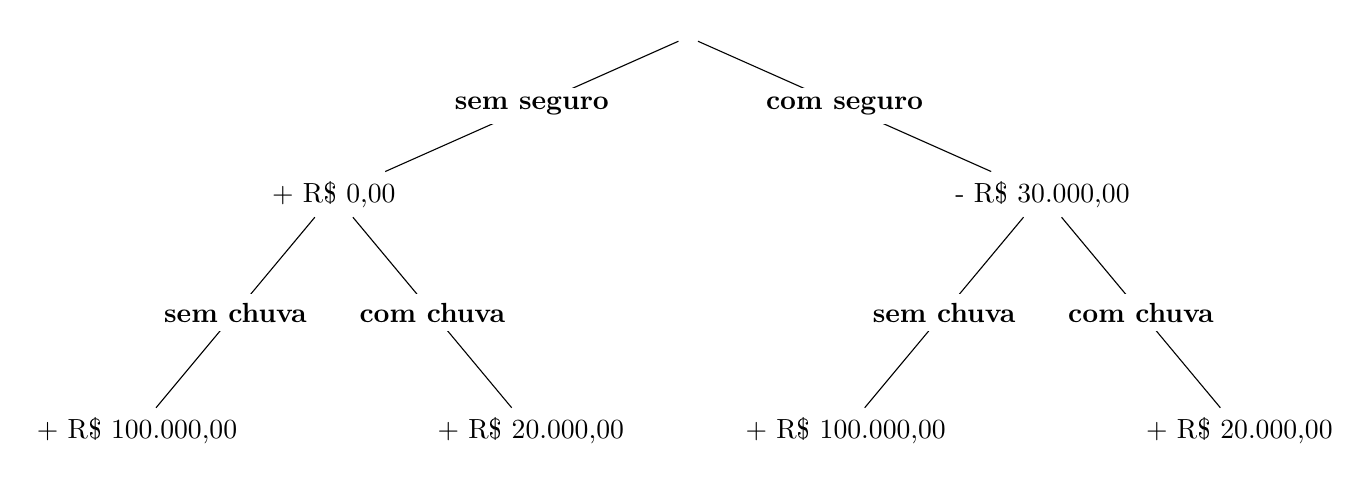
\begin{tikzpicture}
			\tikzstyle{level 1} = [sibling distance=9cm, level distance=2cm]
			\tikzstyle{level 2} = [sibling distance=5cm, level distance=3cm]
			\node{}
			child{
				node{+ R\$ 0,00}
				child{
					node{+ R\$ 100.000,00}
					edge from parent
					node[fill=white]{\textbf{sem chuva}}
				}
				child{
					node{+ R\$ 20.000,00}
					edge from parent
					node[fill=white]{\textbf{com chuva}}
				}
				edge from parent
				node[fill=white]{\textbf{sem seguro}}
			}
			child{
				node{- R\$ 30.000,00}
				child{
					node{+ R\$ 100.000,00}
					edge from parent
					node[fill=white]{\textbf{sem chuva}}
				}
				child{
					node{+ R\$ 20.000,00}
					edge from parent
					node[fill=white]{\textbf{com chuva}}
				}
				edge from parent
				node[fill=white]{\textbf{com seguro}}
			};
		\end{tikzpicture}
		\vspace{1cm}\\
		E$_{1}$(X) = 100 * (1 - p) + 20 * p = 100 - 100p + 20p = - 80p + 100
		\vspace{1cm}\\
		E$_{2}$(X) = (100 - 30) * (1 - p) + (20 + 70 - 30) * p = 70 - 70p + 60p = - 10p + 70
		\vspace{1cm}\\
		E$_{1}$(X) = E$_{2}$(X)
		\vspace{0.25cm}\\
		- 80p + 100 = - 10p + 70
		\vspace{0.25cm}\\
		70p = 30
		\vspace{0.25cm}\\
		p = $\dfrac{3}{7}$
	\end{center}
\end{document}
